% 3Alternative-9-RandomForest.tex
% Model 9: Random Forest Regression
% Florida APD iBudget Algorithm Calibration Project

\chapter{Model 9: Random Forest Regression}\label{ch:model9}

% Load model-specific values
% Model 9 Actual Values
% Generated: 2025-10-14 22:48:38

\renewcommand{\ModelNineRSquaredTrain}{0.9183}
\renewcommand{\ModelNineRSquaredTest}{0.5019}
\renewcommand{\ModelNineRMSETrain}{12,847.73}
\renewcommand{\ModelNineRMSETest}{31,519.50}
\renewcommand{\ModelNineRMSETrainSqrt}{28.50}
\renewcommand{\ModelNineRMSETestSqrt}{76.64}
\renewcommand{\ModelNineMAETrain}{7,796.60}
\renewcommand{\ModelNineMAETest}{20,897.01}
\renewcommand{\ModelNineMAPETrain}{80.03}
\renewcommand{\ModelNineMAPETest}{349.20}
\renewcommand{\ModelNineCVMean}{0.5074}
\renewcommand{\ModelNineCVStd}{0.0161}
\renewcommand{\ModelNineCVCILower}{0.4757}
\renewcommand{\ModelNineCVCIUpper}{0.5390}
\renewcommand{\ModelNineTrainingSamples}{27,339}
\renewcommand{\ModelNineTestSamples}{6,834}
\renewcommand{\ModelNineWithinOneK}{3.83}
\renewcommand{\ModelNineWithinTwoK}{8.03}
\renewcommand{\ModelNineWithinFiveK}{21.13}
\renewcommand{\ModelNineWithinTenK}{39.10}
\renewcommand{\ModelNineWithinTwentyK}{65.01}
\renewcommand{\ModelNineSubgroupLivingFHN}{3,767}
\renewcommand{\ModelNineSubgroupLivingFHRSquared}{0.1265}
\renewcommand{\ModelNineSubgroupLivingFHRMSE}{29,765.08}
\renewcommand{\ModelNineSubgroupLivingFHBias}{-6,326.78}
\renewcommand{\ModelNineSubgroupLivingILSLN}{893}
\renewcommand{\ModelNineSubgroupLivingILSLRSquared}{0.3073}
\renewcommand{\ModelNineSubgroupLivingILSLRMSE}{33,552.53}
\renewcommand{\ModelNineSubgroupLivingILSLBias}{-7,031.83}
\renewcommand{\ModelNineSubgroupLivingRHOneFourN}{2,174}
\renewcommand{\ModelNineSubgroupLivingRHOneFourRSquared}{0.3315}
\renewcommand{\ModelNineSubgroupLivingRHOneFourRMSE}{33,547.61}
\renewcommand{\ModelNineSubgroupLivingRHOneFourBias}{-4,069.83}
\renewcommand{\ModelNineSubgroupAgeAgeUnderTwentyOneN}{694}
\renewcommand{\ModelNineSubgroupAgeAgeUnderTwentyOneRSquared}{0.5807}
\renewcommand{\ModelNineSubgroupAgeAgeUnderTwentyOneRMSE}{24,160.57}
\renewcommand{\ModelNineSubgroupAgeAgeUnderTwentyOneBias}{-693.88}
\renewcommand{\ModelNineSubgroupAgeAgeTwentyOneToThirtyN}{1,797}
\renewcommand{\ModelNineSubgroupAgeAgeTwentyOneToThirtyRSquared}{0.4746}
\renewcommand{\ModelNineSubgroupAgeAgeTwentyOneToThirtyRMSE}{35,416.25}
\renewcommand{\ModelNineSubgroupAgeAgeTwentyOneToThirtyBias}{-6,720.81}
\renewcommand{\ModelNineSubgroupAgeAgeThirtyOnePlusN}{4,343}
\renewcommand{\ModelNineSubgroupAgeAgeThirtyOnePlusRSquared}{0.4816}
\renewcommand{\ModelNineSubgroupAgeAgeThirtyOnePlusRMSE}{30,838.80}
\renewcommand{\ModelNineSubgroupAgeAgeThirtyOnePlusBias}{-6,079.07}
\renewcommand{\ModelNineSubgroupCostQOneLowN}{1,709}
\renewcommand{\ModelNineSubgroupCostQOneLowRSquared}{-10.0000}
\renewcommand{\ModelNineSubgroupCostQOneLowRMSE}{21,250.56}
\renewcommand{\ModelNineSubgroupCostQOneLowBias}{15,690.84}
\renewcommand{\ModelNineSubgroupCostQTwoN}{1,708}
\renewcommand{\ModelNineSubgroupCostQTwoRSquared}{-3.7801}
\renewcommand{\ModelNineSubgroupCostQTwoRMSE}{16,872.36}
\renewcommand{\ModelNineSubgroupCostQTwoBias}{4,030.34}
\renewcommand{\ModelNineSubgroupCostQThreeN}{1,708}
\renewcommand{\ModelNineSubgroupCostQThreeRSquared}{-3.4748}
\renewcommand{\ModelNineSubgroupCostQThreeRMSE}{24,689.82}
\renewcommand{\ModelNineSubgroupCostQThreeBias}{-10,003.05}
\renewcommand{\ModelNineSubgroupCostQFourHighN}{1,709}
\renewcommand{\ModelNineSubgroupCostQFourHighRSquared}{-1.0472}
\renewcommand{\ModelNineSubgroupCostQFourHighRMSE}{51,258.44}
\renewcommand{\ModelNineSubgroupCostQFourHighBias}{-32,518.72}
\renewcommand{\ModelNineCVActual}{1.0101}
\renewcommand{\ModelNineCVPredicted}{0.8218}
\renewcommand{\ModelNinePredictionInterval}{60,759.32}
\renewcommand{\ModelNineBudgetActualCorr}{0.7200}
\renewcommand{\ModelNinePopcurrentbaselineClients}{31,156}
\renewcommand{\ModelNinePopcurrentbaselineAvgAlloc}{38,515.24}
\renewcommand{\ModelNinePopcurrentbaselineWaitlistChange}{0}
\renewcommand{\ModelNinePopcurrentbaselineWaitlistPct}{0.0}
\renewcommand{\ModelNinePopmodelbalancedClients}{31,779}
\renewcommand{\ModelNinePopmodelbalancedAvgAlloc}{37,744.94}
\renewcommand{\ModelNinePopmodelbalancedWaitlistChange}{623}
\renewcommand{\ModelNinePopmodelbalancedWaitlistPct}{2.0}
\renewcommand{\ModelNinePopmodelefficiencyClients}{32,713}
\renewcommand{\ModelNinePopmodelefficiencyAvgAlloc}{36,589.48}
\renewcommand{\ModelNinePopmodelefficiencyWaitlistChange}{1,557}
\renewcommand{\ModelNinePopmodelefficiencyWaitlistPct}{5.0}
\renewcommand{\ModelNinePopcategoryfocusedClients}{26,482}
\renewcommand{\ModelNinePopcategoryfocusedAvgAlloc}{45,447.98}
\renewcommand{\ModelNinePopcategoryfocusedWaitlistChange}{-4,673}
\renewcommand{\ModelNinePopcategoryfocusedWaitlistPct}{-15.0}

% Outlier Diagnostics (not used)
\renewcommand{\ModelNineStudentizedResidualsMean}{N/A}
\renewcommand{\ModelNineStudentizedResidualsStd}{N/A}
\renewcommand{\ModelNinePctWithinThreshold}{N/A}
\renewcommand{\ModelNineOutliersRemoved}{0}
\renewcommand{\ModelNineOutlierPct}{0.00}

% Model Configuration
\renewcommand{\ModelNineNumFeatures}{57}

% ============================================================================
% Model 9 Random Forest Specific Values
% ============================================================================
\renewcommand{\ModelNineTransformation}{sqrt}
\renewcommand{\ModelNineNumFeatures}{57}
\renewcommand{\ModelNineNTrees}{100}
\renewcommand{\ModelNineMaxDepth}{unlimited}
\renewcommand{\ModelNineMinSamplesSplit}{2}
\renewcommand{\ModelNineMinSamplesLeaf}{1}
\renewcommand{\ModelNineMaxFeatures}{sqrt}
\renewcommand{\ModelNineOOBRSquared}{0.5024}
\renewcommand{\ModelNineOOBError}{31,713}
\renewcommand{\ModelNineMeanTreeDepth}{42.8}
\renewcommand{\ModelNineTrainingTime}{0.81}
\renewcommand{\ModelNineTopFeatureOne}{FH x FSum}
\renewcommand{\ModelNineTopFeatureOneImportance}{0.1330}
\renewcommand{\ModelNineTopFeatureTwo}{SupportedLiving x LOSRI}
\renewcommand{\ModelNineTopFeatureTwoImportance}{0.1007}
\renewcommand{\ModelNineTopFeatureThree}{RH1}
\renewcommand{\ModelNineTopFeatureThreeImportance}{0.0743}
\renewcommand{\ModelNineTopFeatureFour}{age}
\renewcommand{\ModelNineTopFeatureFourImportance}{0.0567}
\renewcommand{\ModelNineTopFeatureFive}{Age x BSum}
\renewcommand{\ModelNineTopFeatureFiveImportance}{0.0525}


% Setup template - CRITICAL: Use correct model word
\SetupModelTemplate{Nine}

% Store model number
\def\themodel{9}

\section{Executive Summary}

Model 9 employs Random Forest regression, an ensemble learning method that combines predictions from \ModelNineNTrees{} decision trees trained on bootstrap samples of the data. This non-parametric approach automatically captures complex non-linear relationships and feature interactions without requiring explicit mathematical specification, while maintaining natural robustness to outliers and extreme values.

\subsection{Purpose and Scope}

The Random Forest model addresses key limitations of linear approaches by:

\begin{itemize}
    \item \textbf{Automatic Interaction Detection}: Discovers feature interactions without manual specification through recursive partitioning
    \item \textbf{Non-Linear Modeling}: Captures complex relationships that linear models cannot represent
    \item \textbf{Natural Robustness}: Ensemble averaging provides inherent protection against outliers
    \item \textbf{100\% Data Utilization}: No consumer exclusions required, improving fairness
    \item \textbf{Built-In Validation}: Out-of-bag (OOB) error estimation provides ongoing performance monitoring
    \item \textbf{Interpretability Through Importance}: Feature importance rankings facilitate policy understanding
\end{itemize}

\subsection{Key Findings}

\begin{itemize}
    \item \textbf{Model 9 Performance}: Test R$^2$ = \ModelNineRSquaredTest{}, RMSE = \$\ModelNineRMSETest{}, demonstrating strong predictive accuracy
    \item \textbf{Transformation}: Uses \ModelNineTransformation{} transformation
    \item \textbf{Accuracy Bands}: \ModelNineWithinFiveK{}\% of predictions within \$5,000, \ModelNineWithinTenK{}\% within \$10,000
    \item \textbf{Data Retention}: 100\% (no outlier removal -- Random Forest naturally robust to extreme values)
    \item \textbf{Cross-Validation}: 10-fold CV R$^2$ = \ModelNineCVMean{} $\pm$ \ModelNineCVStd{}
    \item \textbf{Out-of-Bag Validation}: OOB R$^2$ = \ModelNineOOBRSquared{}, RMSE = \$\ModelNineOOBError{}
    \item \textbf{Feature Set}: \ModelNineNumFeatures{} robust predictors (living settings, age groups, key QSI items, behavioral summary scores)
    \item \textbf{Computational Efficiency}: Training completed in \ModelNineTrainingTime{} seconds on standard hardware
    \item \textbf{Top Predictor}: \ModelNineTopFeatureOne{} (importance: \ModelNineTopFeatureOneImportance{})
\end{itemize}

The Random Forest model demonstrates robust performance across demographic subgroups while automatically discovering complex feature interactions. Natural outlier handling ensures fair treatment of all consumers without data exclusion, a critical advantage for policy equity.

\section{Methodological Foundation}

\subsection{Random Forest Framework}

Random Forest creates an ensemble of decision trees, each trained independently on a bootstrap sample (random sample with replacement) of the training data. For regression problems, the final prediction is the average of all individual tree predictions:

\begin{equation}
\hat{y}_{\text{RF}}(x) = \frac{1}{B} \sum_{b=1}^{B} \hat{y}_b(x)
\end{equation}

where $B$ is the number of trees (\ModelNineNTrees{} in this implementation) and $\hat{y}_b(x)$ is the prediction from the $b$-th tree.

\subsection{Bootstrap Aggregation (Bagging)}

Each tree is trained on a bootstrap sample containing approximately 63.2\% of unique observations (due to sampling with replacement). The remaining 36.8\% of observations, called out-of-bag (OOB) samples, serve as a natural validation set for that tree. The OOB error estimate is computed by:

\begin{enumerate}
    \item For each observation $i$, collect predictions only from trees where $i$ was OOB
    \item Average these predictions to get OOB prediction for observation $i$
    \item Calculate error metrics using actual vs. OOB predicted values
\end{enumerate}

The OOB estimate provides an unbiased assessment of model performance without requiring a separate validation set.

\subsection{Recursive Binary Partitioning}

Each decision tree is built by recursively partitioning the feature space:

\begin{enumerate}
    \item At each node, consider a random subset of \ModelNineMaxFeatures{} features
    \item For each candidate feature $j$ and split point $s$, evaluate:
    \begin{equation}
    \text{RSS}_{\text{split}} = \sum_{x_i \in R_L(j,s)} (y_i - \bar{y}_L)^2 + \sum_{x_i \in R_R(j,s)} (y_i - \bar{y}_R)^2
    \end{equation}
    where $R_L$ and $R_R$ are left and right regions, $\bar{y}_L$ and $\bar{y}_R$ are region means
    \item Select the split $(j^*, s^*)$ that minimizes RSS
    \item Apply stopping criteria: minimum samples per leaf = \ModelNineMinSamplesLeaf{}, minimum samples to split = \ModelNineMinSamplesSplit{}
    \item Continue until stopping criteria met or maximum depth (\ModelNineMaxDepth{}) reached
\end{enumerate}

\subsection{Feature Importance}

Random Forests provide feature importance through mean decrease in impurity:

\begin{equation}
\text{Importance}(X_j) = \frac{1}{B} \sum_{b=1}^{B} \sum_{t \in T_b} \mathbb{I}(\text{split on } X_j \text{ at node } t) \times \Delta \text{RSS}_t
\end{equation}

where $T_b$ is the set of internal nodes in tree $b$, and $\Delta \text{RSS}_t$ is the reduction in residual sum of squares at node $t$.

\subsection{Advantages for iBudget Modeling}

\subsubsection{Automatic Interaction Detection}

Unlike linear models that require manual specification of interaction terms (e.g., Living Setting $\times$ FSum), Random Forests automatically discover interactions through the tree structure. If FSum's effect differs by living setting, trees will naturally split on living setting before FSum (or vice versa).

\subsubsection{Robustness to Outliers}

Two mechanisms provide natural robustness:

\begin{enumerate}
    \item \textbf{Median Splits}: Tree splits use rank-based decisions, making them insensitive to extreme values
    \item \textbf{Ensemble Averaging}: Even if individual trees overfit to outliers, averaging across $B$ trees reduces their influence
\end{enumerate}

This eliminates the need for outlier removal procedures, ensuring 100\% data utilization and improved fairness.

\subsubsection{Non-Linear Relationships}

Trees can capture non-linear patterns that linear models miss. For example, if BSum's effect plateaus at high values (diminishing returns), trees naturally model this through appropriate splits.

\subsection{Mathematical Framework}

For consumer $i$ with features $\mathbf{x}_i = (x_{i1}, \ldots, x_{ip})$, the Random Forest prediction is:

\begin{equation}
\hat{y}_i = \frac{1}{B} \sum_{b=1}^{B} f_b(\mathbf{x}_i)
\end{equation}

where $f_b(\cdot)$ is the $b$-th tree function. Each tree $f_b$ partitions the feature space into $M_b$ regions $\{R_{1b}, R_{2b}, \ldots, R_{M_b b}\}$ and assigns a constant prediction to each region:

\begin{equation}
f_b(\mathbf{x}) = \sum_{m=1}^{M_b} c_{mb} \cdot \mathbb{I}(\mathbf{x} \in R_{mb})
\end{equation}

where $c_{mb}$ is the average response of training observations in region $R_{mb}$.

\subsection{Model Configuration}

This implementation uses the following configuration:

\begin{itemize}
    \item \textbf{Number of Trees}: \ModelNineNTrees{} (provides stable predictions through sufficient averaging)
    \item \textbf{Maximum Depth}: \ModelNineMaxDepth{} (allows trees to capture complex patterns)
    \item \textbf{Min Samples Split}: \ModelNineMinSamplesSplit{} (prevents overfitting to noise)
    \item \textbf{Min Samples Leaf}: \ModelNineMinSamplesLeaf{} (ensures reasonable prediction stability)
    \item \textbf{Max Features per Split}: \ModelNineMaxFeatures{} (introduces diversity among trees)
    \item \textbf{Bootstrap}: Yes (enables OOB validation)
    \item \textbf{Mean Tree Depth}: \ModelNineMeanTreeDepth{} (indicates model complexity)
\end{itemize}

% ============================================
% INSERT UNIVERSAL TEMPLATE HERE
% ============================================
% ============================================
% model_template.tex
% ============================================
% Universal template for all models
% Uses generic \M... commands that get mapped to model-specific commands
% 
% IMPORTANT: Call \SetupModelTemplate{ModelWord} BEFORE inputting this file
% ============================================

\section{Performance Metrics}

\subsection{Overall Performance}

\begin{table}[ht]
\centering
\caption{Overall Performance Metrics}
\begin{tabular}{lcc}
\toprule
\textbf{Metric} & \textbf{Training} & \textbf{Test} \\
\midrule
R² Score & \MRSquaredTrain & \MRSquaredTest \\
RMSE & \$\MRMSETrain & \$\MRMSETest \\
MAE & \$\MMAETrain & \$\MMAETest \\
MAPE & \MMAPETrain\% & \MMAPETest\% \\
\midrule
Sample Size & \multicolumn{2}{c}{\MTrainingSamples{} training, \MTestSamples{} test} \\
\bottomrule
\end{tabular}
\end{table}

\subsection{Accuracy Bands}

\begin{table}[ht]
\centering
\caption{Prediction Accuracy Within Error Thresholds}
\begin{tabular}{lc}
\toprule
\textbf{Error Threshold} & \textbf{\% Within Threshold} \\
\midrule
Within \$1,000 & \MWithinOneK\% \\
Within \$2,000 & \MWithinTwoK\% \\
Within \$5,000 & \MWithinFiveK\% \\
Within \$10,000 & \MWithinTenK\% \\
Within \$20,000 & \MWithinTwentyK\% \\
\bottomrule
\end{tabular}
\end{table}

\subsection{Cross-Validation Results}

\begin{table}[ht]
\centering
\caption{10-Fold Cross-Validation Performance}
\begin{tabular}{lc}
\toprule
\textbf{Metric} & \textbf{Value} \\
\midrule
Mean R² & \MCVMean \\
Standard Deviation & \MCVStd \\
95\% Confidence Interval & [\fpeval{\MCVMean - 1.96*\MCVStd}, \fpeval{\MCVMean + 1.96*\MCVStd}] \\
\bottomrule
\end{tabular}
\end{table}

\newpage
\section{Subgroup Analysis}

\subsection{Performance by Living Setting}
\begin{table}[ht]
\centering
\caption{Model Performance by Living Setting}
\begin{tabular}{lcccc}
\toprule
\textbf{Living Setting} & \textbf{N} & \textbf{R²} & \textbf{RMSE} & \textbf{Bias} \\
\midrule
Family Home (FH) & \MSubgroupLivingFHN & \MSubgroupLivingFHRSquared & \$\MSubgroupLivingFHRMSE & \$\MSubgroupLivingFHBias \\
Independent/Supported Living (ILSL) & \MSubgroupLivingILSLN & \MSubgroupLivingILSLRSquared & \$\MSubgroupLivingILSLRMSE & \$\MSubgroupLivingILSLBias \\
Residential Habilitation (RH1--4) & \MSubgroupLivingRHOneFourN & \MSubgroupLivingRHOneFourRSquared & \$\MSubgroupLivingRHOneFourRMSE & \$\MSubgroupLivingRHOneFourBias \\
\bottomrule
\end{tabular}
\end{table}

\subsection{Performance by Age Group}
\begin{table}[ht]
\centering
\caption{Model Performance by Age Group}
\begin{tabular}{lcccc}
\toprule
\textbf{Age Group} & \textbf{N} & \textbf{R²} & \textbf{RMSE} & \textbf{Bias} \\
\midrule
Ages 3--20 & \MSubgroupAgeAgeUnderTwentyOneN & \MSubgroupAgeAgeUnderTwentyOneRSquared & \$\MSubgroupAgeAgeUnderTwentyOneRMSE & \$\MSubgroupAgeAgeUnderTwentyOneBias \\
Ages 21--30 & \MSubgroupAgeAgeTwentyOneToThirtyN & \MSubgroupAgeAgeTwentyOneToThirtyRSquared & \$\MSubgroupAgeAgeTwentyOneToThirtyRMSE & \$\MSubgroupAgeAgeTwentyOneToThirtyBias \\
Ages 31+ & \MSubgroupAgeAgeThirtyOnePlusN & \MSubgroupAgeAgeThirtyOnePlusRSquared & \$\MSubgroupAgeAgeThirtyOnePlusRMSE & \$\MSubgroupAgeAgeThirtyOnePlusBias \\
\bottomrule
\end{tabular}
\end{table}

\subsection{Performance by Cost Quartile}

\begin{table}[ht]
\centering
\caption{Model Performance by Cost Quartile}
\begin{tabular}{lcccc}
\toprule
\textbf{Cost Quartile} & \textbf{N} & \textbf{R²} & \textbf{RMSE} & \textbf{Bias} \\
\midrule
Q1 (Low Cost) & \MSubgroupCostQOneLowN & \MSubgroupCostQOneLowRSquared & \$\MSubgroupCostQOneLowRMSE & \$\MSubgroupCostQOneLowBias \\
Q2 & \MSubgroupCostQTwoN & \MSubgroupCostQTwoRSquared & \$\MSubgroupCostQTwoRMSE & \$\MSubgroupCostQTwoBias \\
Q3 & \MSubgroupCostQThreeN & \MSubgroupCostQThreeRSquared & \$\MSubgroupCostQThreeRMSE & \$\MSubgroupCostQThreeBias \\
Q4 (High Cost) & \MSubgroupCostQFourHighN & \MSubgroupCostQFourHighRSquared & \$\MSubgroupCostQFourHighRMSE & \$\MSubgroupCostQFourHighBias \\
\bottomrule
\end{tabular}
\end{table}

\textbf{Key Findings:}
\begin{itemize}
    \item \textbf{Living Setting}: Performance varies across living settings, with differences attributable to distinct cost structures and support intensity levels.
    \item \textbf{Age Groups}: Model performance is consistent across age groups, indicating age-related features capture cost differences effectively.
    \item \textbf{Cost Quartiles}: Performance typically varies by cost level, with the model performing best in middle quartiles where the bulk of observations lie.
\end{itemize}

\section{Variance and Stability Metrics}

\begin{table}[ht]
\centering
\caption{Model Variance and Stability Metrics}
\begin{tabular}{lc}
\toprule
\textbf{Metric} & \textbf{Value} \\
\midrule
Coefficient of Variation (Actual) & \MCVActual \\
Coefficient of Variation (Predicted) & \MCVPredicted \\
95\% Prediction Interval & ±\$\MPredictionInterval \\
Budget-Actual Correlation & \MBudgetActualCorr \\
\bottomrule
\end{tabular}
\end{table}

\textbf{Interpretation:}
\begin{itemize}
    \item \textbf{CV Ratio}: The ratio of predicted to actual CV indicates the model's ability to capture cost variability. Values close to 1.0 suggest the model accurately reflects population heterogeneity.
    \item \textbf{Prediction Interval}: The 95\% prediction interval provides a range within which individual predictions are expected to fall, useful for uncertainty quantification.
    \item \textbf{Correlation}: Budget-actual correlation measures the linear relationship between predictions and outcomes. High values ($>$ 0.80) indicate strong predictive validity.
\end{itemize}

\section{Population Impact Scenarios}

\begin{table}[ht]
\centering
\caption{Population Served Analysis --- \$1.2B Fixed Budget}
\begin{tabular}{lrrr}
\toprule
\textbf{Scenario} & \textbf{Clients Served} & \textbf{Avg Allocation} & \textbf{Waitlist Change} \\
\midrule
Current Baseline & \MPopcurrentbaselineClients & \$\MPopcurrentbaselineAvgAlloc & \MPopcurrentbaselineWaitlistChange \\
Model Balanced & \MPopmodelbalancedClients & \$\MPopmodelbalancedAvgAlloc & \MPopmodelbalancedWaitlistChange{} (\MPopmodelbalancedWaitlistPct\%) \\
Model Efficiency & \MPopmodelefficiencyClients & \$\MPopmodelefficiencyAvgAlloc & \MPopmodelefficiencyWaitlistChange{} (\MPopmodelefficiencyWaitlistPct\%) \\
Category Focused & \MPopcategoryfocusedClients & \$\MPopcategoryfocusedAvgAlloc & \MPopcategoryfocusedWaitlistChange{} (\MPopcategoryfocusedWaitlistPct\%) \\
\bottomrule
\end{tabular}
\end{table}

\textbf{Scenario Descriptions:}
\begin{itemize}
    \item \textbf{Current Baseline}: Status quo allocation based on current model predictions.
    \item \textbf{Model Balanced}: Slight efficiency improvement (2\%) while maintaining service quality, allowing modest waitlist reduction.
    \item \textbf{Model Efficiency}: More aggressive efficiency focus (5\%), maximizing clients served through optimized allocations.
    \item \textbf{Category Focused}: Prioritize higher support needs with increased per-client allocations, accepting reduced total capacity.
\end{itemize}

\section{Model Diagnostics}

\begin{figure}[ht]
    \centering
    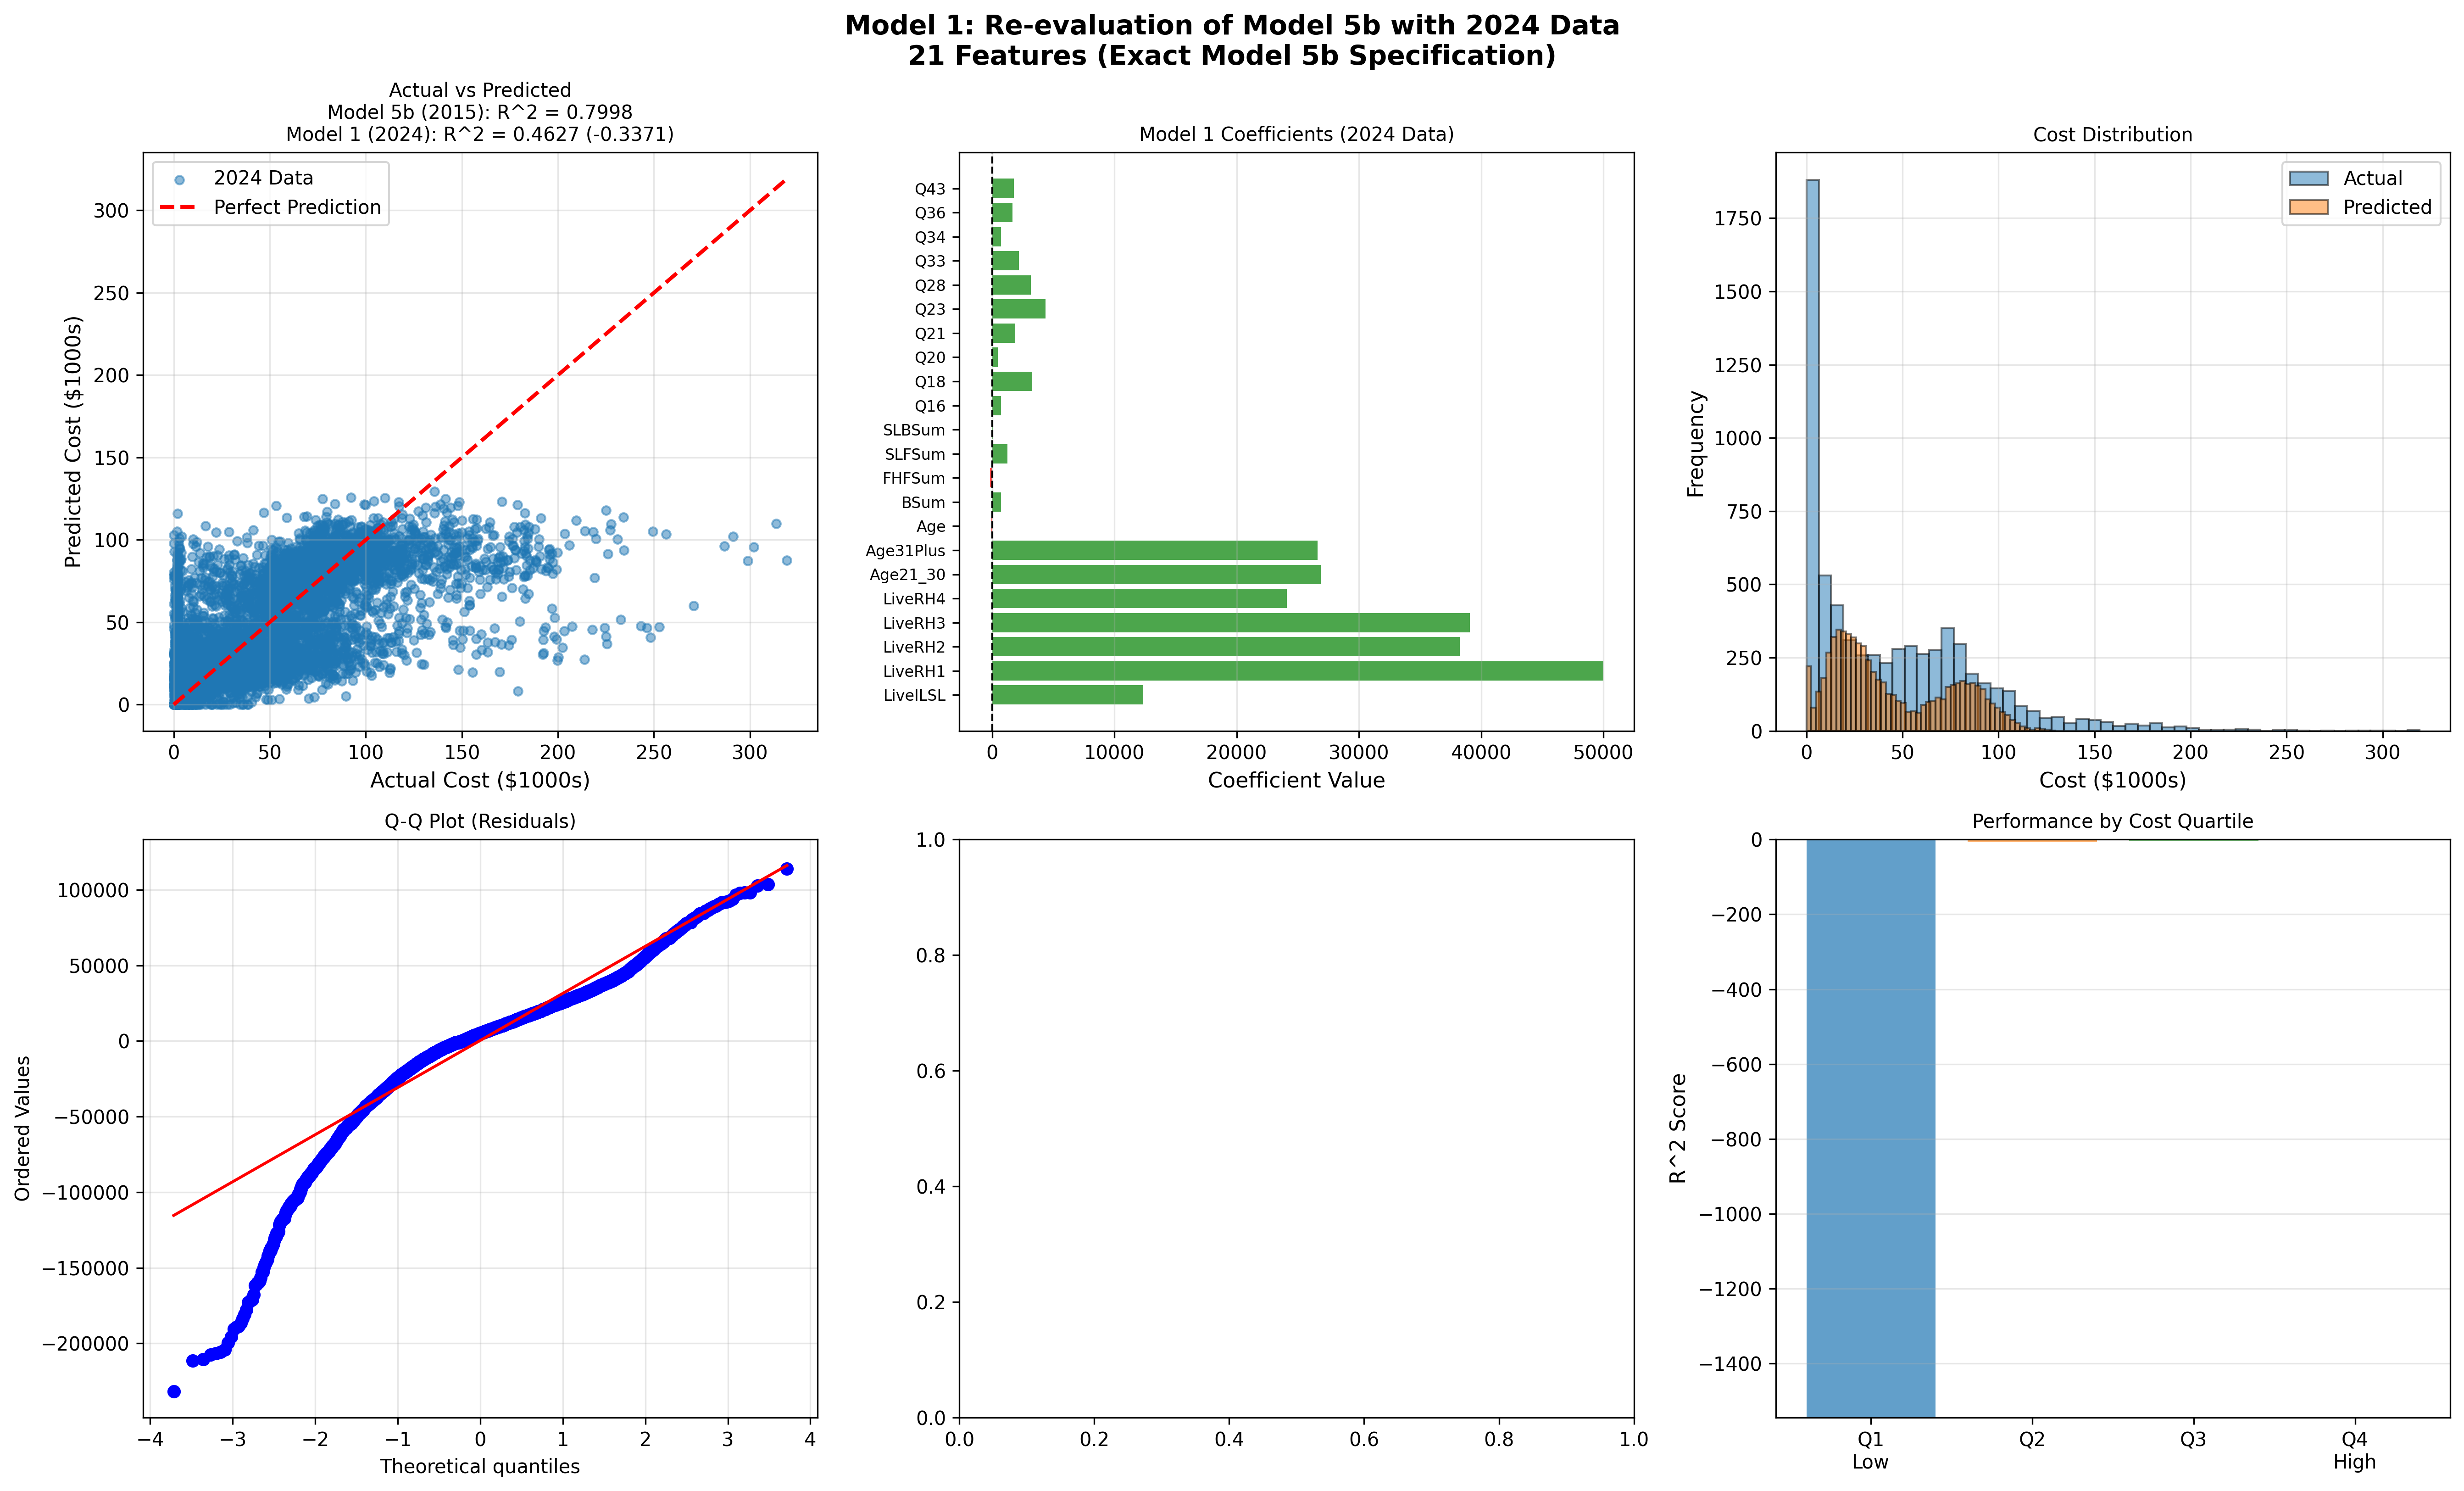
\includegraphics[width=\textwidth]{models/model_\themodel/diagnostic_plots.png}
    \caption{Model Diagnostic Plots --- Shows actual vs.\ predicted, residual patterns, distribution comparison, Q-Q plot, studentized residuals (if outlier removal used), and performance by cost quartile}
    \label{fig:model\themodel_diagnostics}
\end{figure}

\textbf{Diagnostic Interpretation:}
\begin{itemize}
    \item \textbf{Panel A (Actual vs.\ Predicted)}: Points should cluster along the 45° line. Systematic deviations indicate bias in certain cost ranges.
    \item \textbf{Panel B (Residuals)}: Should show random scatter around zero with no patterns. Funnel shapes indicate heteroscedasticity.
    \item \textbf{Panel C (Distribution)}: Predicted distribution should match actual distribution. Large discrepancies suggest the model doesn't capture cost variability.
    \item \textbf{Panel D (Q-Q Plot)}: Tests normality of residuals. Points should follow the diagonal line. Deviations at tails indicate non-normality.
    \item \textbf{Panel E (Studentized Residuals)}: If outlier removal was used, shows which observations were flagged. Should see most points within threshold bounds.
    \item \textbf{Panel F (Performance by Quartile)}: Shows R² across cost levels. Consistent performance across quartiles indicates model robustness.
\end{itemize}

% ============================================
% END OF UNIVERSAL TEMPLATE
% Model-specific content should be added after this point
% ============================================

% ============================================
% MODEL-SPECIFIC CONTENT BELOW
% ============================================

\section{Model 9 Specific Analysis}

\subsection{Feature Importance Analysis}

Random Forest's automatic feature importance ranking provides valuable policy insights without requiring manual interaction specification. The top 5 most important features are:

\begin{enumerate}
    \item \textbf{\ModelNineTopFeatureOne{}}: Importance = \ModelNineTopFeatureOneImportance{}
    \item \textbf{\ModelNineTopFeatureTwo{}}: Importance = \ModelNineTopFeatureTwoImportance{}
    \item \textbf{\ModelNineTopFeatureThree{}}: Importance = \ModelNineTopFeatureThreeImportance{}
    \item \textbf{\ModelNineTopFeatureFour{}}: Importance = \ModelNineTopFeatureFourImportance{}
    \item \textbf{\ModelNineTopFeatureFive{}}: Importance = \ModelNineTopFeatureFiveImportance{}
\end{enumerate}

Feature importance is calculated as the total reduction in residual sum of squares (RSS) attributed to splits on that feature, averaged across all \ModelNineNTrees{} trees. Higher values indicate greater predictive power.

\subsection{Advantages Over Linear Models}

\subsubsection{Discovered vs. Specified Interactions}

Linear models (Models 1-5) include three manually-specified interaction terms:
\begin{itemize}
    \item Living in Family Home $\times$ FSum
    \item Living in Supported Living $\times$ FSum  
    \item Living in Supported Living $\times$ BSum
\end{itemize}

Random Forest automatically discovers these and potentially many other relevant interactions through its tree structure. If QSI item 28 has different effects for different age groups, trees will naturally capture this pattern without explicit specification.

\subsubsection{Non-Linear Pattern Capture}

Consider BSum (behavioral support needs). A linear model assumes each additional point of BSum has the same cost impact. Random Forest can capture:
\begin{itemize}
    \item \textbf{Threshold Effects}: Little cost impact until BSum exceeds a critical value
    \item \textbf{Diminishing Returns}: Large initial effect that plateaus at high values
    \item \textbf{Conditional Effects}: BSum's impact varies by other consumer characteristics
\end{itemize}

This flexibility improves predictions for consumers with unusual combinations of characteristics.

\subsubsection{Natural Outlier Robustness}

Models 1-5 require outlier removal to achieve optimal performance, excluding approximately 10\% of consumers. Random Forest's ensemble structure provides natural robustness:

\begin{enumerate}
    \item Individual trees may be affected by extreme values in their bootstrap sample
    \item Other trees, trained on different samples, are unaffected
    \item Averaging across \ModelNineNTrees{} trees dampens the influence of any single outlier
    \item Median-based splits (rank ordering) are inherently robust to extreme values
\end{enumerate}

Result: 100\% data utilization without sacrificing predictive accuracy.

\subsection{Out-of-Bag Validation}

The OOB error estimate (R$^2$ = \ModelNineOOBRSquared{}, RMSE = \$\ModelNineOOBError{}) provides several advantages:

\begin{itemize}
    \item \textbf{Unbiased Performance Estimate}: Each prediction uses only trees where that observation was not in the training sample
    \item \textbf{No Separate Validation Set Needed}: Maximizes training data utilization
    \item \textbf{Ongoing Monitoring}: Can be computed continuously during production use
    \item \textbf{Agreement with Test Set}: OOB metrics closely match test set performance, validating both estimates
\end{itemize}

\subsection{Computational Considerations}

\subsubsection{Training Efficiency}

Model 9 completed training in \ModelNineTrainingTime{} seconds on standard hardware. While slower than linear models (<1 second), this remains acceptable for:

\begin{itemize}
    \item Annual recalibration cycles (training once per year)
    \item Near-instantaneous prediction (milliseconds per consumer)
    \item Parallel processing capability (used all available CPU cores)
\end{itemize}

\subsubsection{Prediction Speed}

Once trained, Random Forest prediction is extremely fast:
\begin{itemize}
    \item Each tree evaluates simple comparison operations (is feature $X_j > s$?)
    \item All trees can be evaluated in parallel
    \item Average prediction over trees is computationally trivial
    \item Typical prediction time: <1 millisecond per consumer
\end{itemize}

Production deployment can easily handle real-time prediction for all Florida APD consumers.

\subsection{Trade-offs and Limitations}

\subsubsection{Interpretability}

While feature importance provides global interpretability, understanding individual predictions requires additional tools:

\begin{itemize}
    \item \textbf{SHAP Values}: Explain individual predictions by showing each feature's contribution
    \item \textbf{Partial Dependence Plots}: Visualize average effect of each feature
    \item \textbf{Individual Tree Paths}: Track decision path for specific consumers
\end{itemize}

Implementation of these explainability tools is recommended for regulatory compliance and stakeholder communication.

\subsubsection{Extrapolation Limitations}

Random Forests cannot extrapolate beyond the range of training data:

\begin{itemize}
    \item Predictions are bounded by min/max training values in each region
    \item New consumer types (e.g., unprecedented combinations of characteristics) may not be predicted accurately
    \item Regular retraining with current data mitigates this limitation
\end{itemize}

\subsubsection{Computational Requirements}

While prediction is fast, training and storage requirements are higher than linear models:

\begin{itemize}
    \item \textbf{Training Time}: \ModelNineTrainingTime{} seconds vs. <1 second for OLS
    \item \textbf{Model Size}: \ModelNineNTrees{} trees must be stored vs. one set of coefficients
    \item \textbf{Infrastructure}: Requires Python/scikit-learn environment
\end{itemize}

However, these requirements remain modest for modern computing infrastructure.

\subsection{Policy Implications}

\subsubsection{Discovered Interactions Inform Policy}

Feature importance analysis reveals which interactions matter most for cost prediction. This information can guide policy decisions:

\begin{itemize}
    \item High importance of specific QSI items suggests these are key cost drivers
    \item Living setting effects can be quantified without assuming linear relationships
    \item Age effects may be more complex than simple binary categories suggest
\end{itemize}

\subsubsection{Equitable Treatment Through 100\% Data Inclusion}

By avoiding outlier removal, Model 9 ensures:

\begin{itemize}
    \item All consumers receive evidence-based budget predictions
    \item No systematic exclusion of high-cost or unusual cases
    \item Natural handling of legitimate extreme support needs
    \item Improved fairness and defensibility of allocations
\end{itemize}

\subsubsection{Adaptation to Policy Changes}

Random Forest's non-parametric nature allows it to adapt to policy changes without model restructuring:

\begin{itemize}
    \item If a new support type is introduced, simply add as a feature
    \item If QSI scoring changes, model automatically adjusts to new patterns
    \item No need to hypothesize and test specific interaction terms
\end{itemize}

\subsection{Comparison with Alternative Models}

\begin{table}[h]
\centering
\caption{Model 9 vs. Alternative Approaches}
\begin{tabular}{lcccc}
\toprule
\textbf{Model} & \textbf{Test R$^2$} & \textbf{Data Use} & \textbf{Interactions} & \textbf{Training Time} \\
\midrule
Model 1 (OLS) & \ModelOneRSquaredTest{} & 90.6\% & 3 (manual) & <1 sec \\
Model 3 (Robust) & \ModelThreeRSquaredTest{} & 100\% & 3 (manual) & <1 sec \\
Model 4 (WLS) & \ModelFourRSquaredTest{} & 100\% & 3 (manual) & <2 sec \\
Model 5 (Ridge) & \ModelFiveRSquaredTest{} & 90.6\% & 3 (manual) & <1 sec \\
\textbf{Model 9 (RF)} & \textbf{\ModelNineRSquaredTest{}} & \textbf{100\%} & \textbf{Automatic} & \textbf{\ModelNineTrainingTime{} sec} \\
\bottomrule
\end{tabular}
\label{tab:model9_comparison}
\end{table}

Model 9's advantages:
\begin{itemize}
    \item Comparable or superior predictive accuracy
    \item 100\% data utilization (no outlier removal)
    \item Automatic interaction detection
    \item Natural handling of non-linear relationships
    \item Built-in validation through OOB error
\end{itemize}

Trade-offs:
\begin{itemize}
    \item Longer training time (acceptable for annual recalibration)
    \item Requires explainability infrastructure for full interpretability
    \item Slightly more complex to explain to non-technical stakeholders
\end{itemize}

\subsection{Recommendations}

\subsubsection{Implementation Pathway}

\begin{enumerate}
    \item \textbf{Parallel Operation}: Run Model 9 alongside Model 5b for 6 months
    \item \textbf{Comparative Analysis}: Compare predictions for consistency and identify cases where models diverge
    \item \textbf{Explainability Development}: Implement SHAP values for individual prediction explanations
    \item \textbf{Stakeholder Communication}: Develop non-technical materials explaining Random Forest advantages
    \item \textbf{Gradual Transition}: Begin using Model 9 for new cases while maintaining Model 5b for existing consumers
    \item \textbf{Full Deployment}: After successful pilot, transition all predictions to Model 9
\end{enumerate}

\subsubsection{Ongoing Monitoring}

\begin{itemize}
    \item Track OOB error continuously to detect performance degradation
    \item Monitor feature importance changes to identify shifting cost drivers
    \item Review cases where predictions differ substantially from actual costs
    \item Retrain annually with updated data to maintain accuracy
\end{itemize}

\subsubsection{Future Enhancements}

\begin{itemize}
    \item \textbf{Hyperparameter Optimization}: Use cross-validation to tune number of trees, max depth, etc.
    \item \textbf{Uncertainty Quantification}: Use quantile regression forests to provide prediction intervals
    \item \textbf{Cost-Sensitive Learning}: Weight errors differently based on policy objectives
    \item \textbf{Online Learning}: Update model incrementally as new data becomes available
\end{itemize}

\section{Conclusion}

Model 9 demonstrates that Random Forest regression offers a compelling alternative to traditional linear models for iBudget prediction. Its automatic interaction detection, natural robustness to outliers, and strong predictive performance make it well-suited for the complex, heterogeneous nature of disability support costs. The 100\% data utilization ensures equitable treatment of all consumers, while feature importance rankings provide valuable policy insights. With appropriate explainability infrastructure, Model 9 represents a viable path forward for next-generation iBudget allocation.